\section{Problems}

\subsection{Question One}
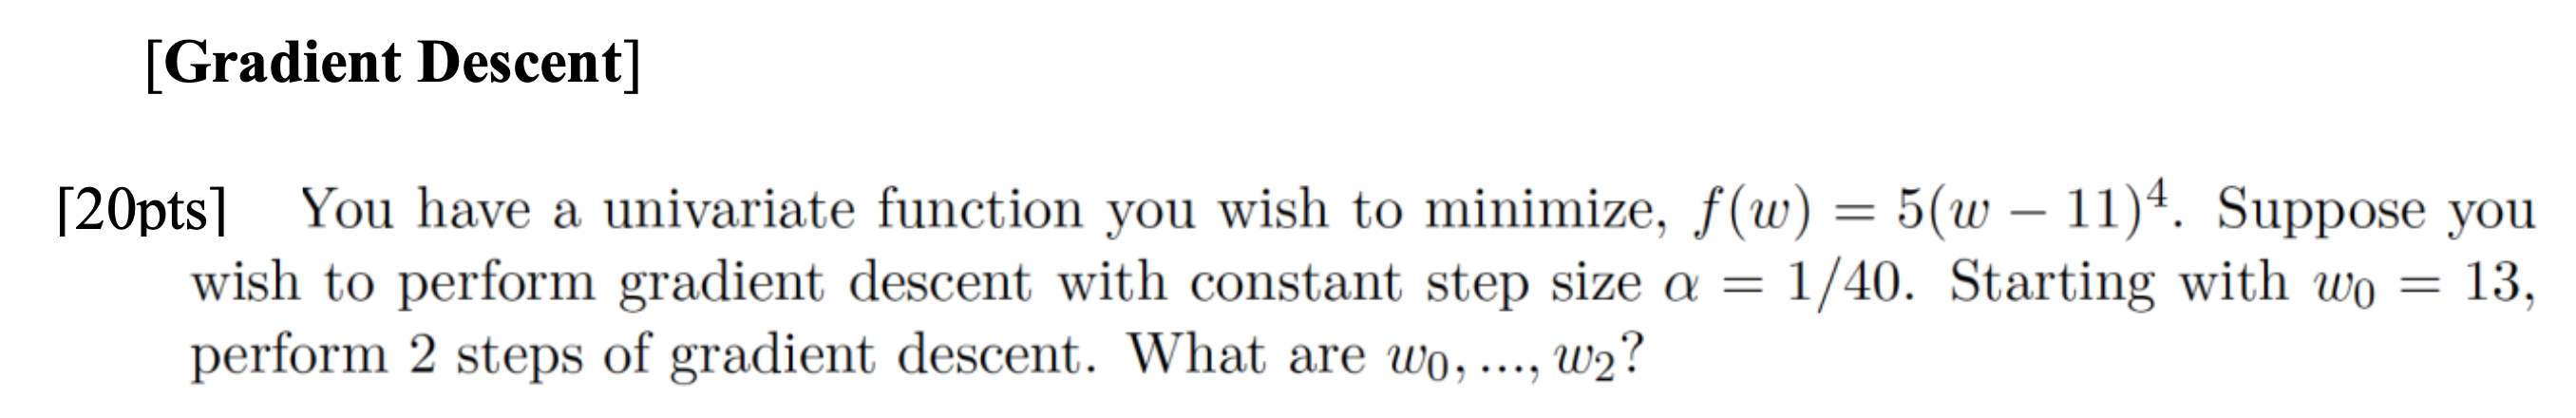
\includegraphics[width=1\textwidth]{media/hw4_q1.png}

Let's start by taking the derivative of $f(w)$:

\begin{align}
    \nabla_w f(w) &= 20(w-11)^3 \label{eq:q1_1}
\end{align}

Gradient descent is given by:
\begin{enumerate}
    \item Initialize $x \leftarrow x_0$
    \item $x \leftarrow x - \alpha \nabla_x f(x)$
    \item repeat until convergence
\end{enumerate}

So for our first step of gradient descent, we have:
\begin{align}
    w &= w_0 = 13 \label{eq:q1_2} \nonumber \\
    w_1 &= w - \alpha \nabla_w f(w) \nonumber \\
    &= 13 - \frac{1}{40} \cdot 20(13-11)^3 \nonumber \\
    &= 9
\end{align}

For our second step of gradient descent, we have:
\begin{align}
    w &= w_1 = 9 \label{eq:q1_3} \nonumber \\
    w_2 &= w - \alpha \nabla_w f(w) \nonumber \\
    &= 9 - \frac{1}{40} \cdot 20(9-11)^3 \nonumber \\
    &= 13
\end{align}

$\therefore \{w_0, w_1, w_2\} = \{13,9,13\}$.

\subsection{Question Two}
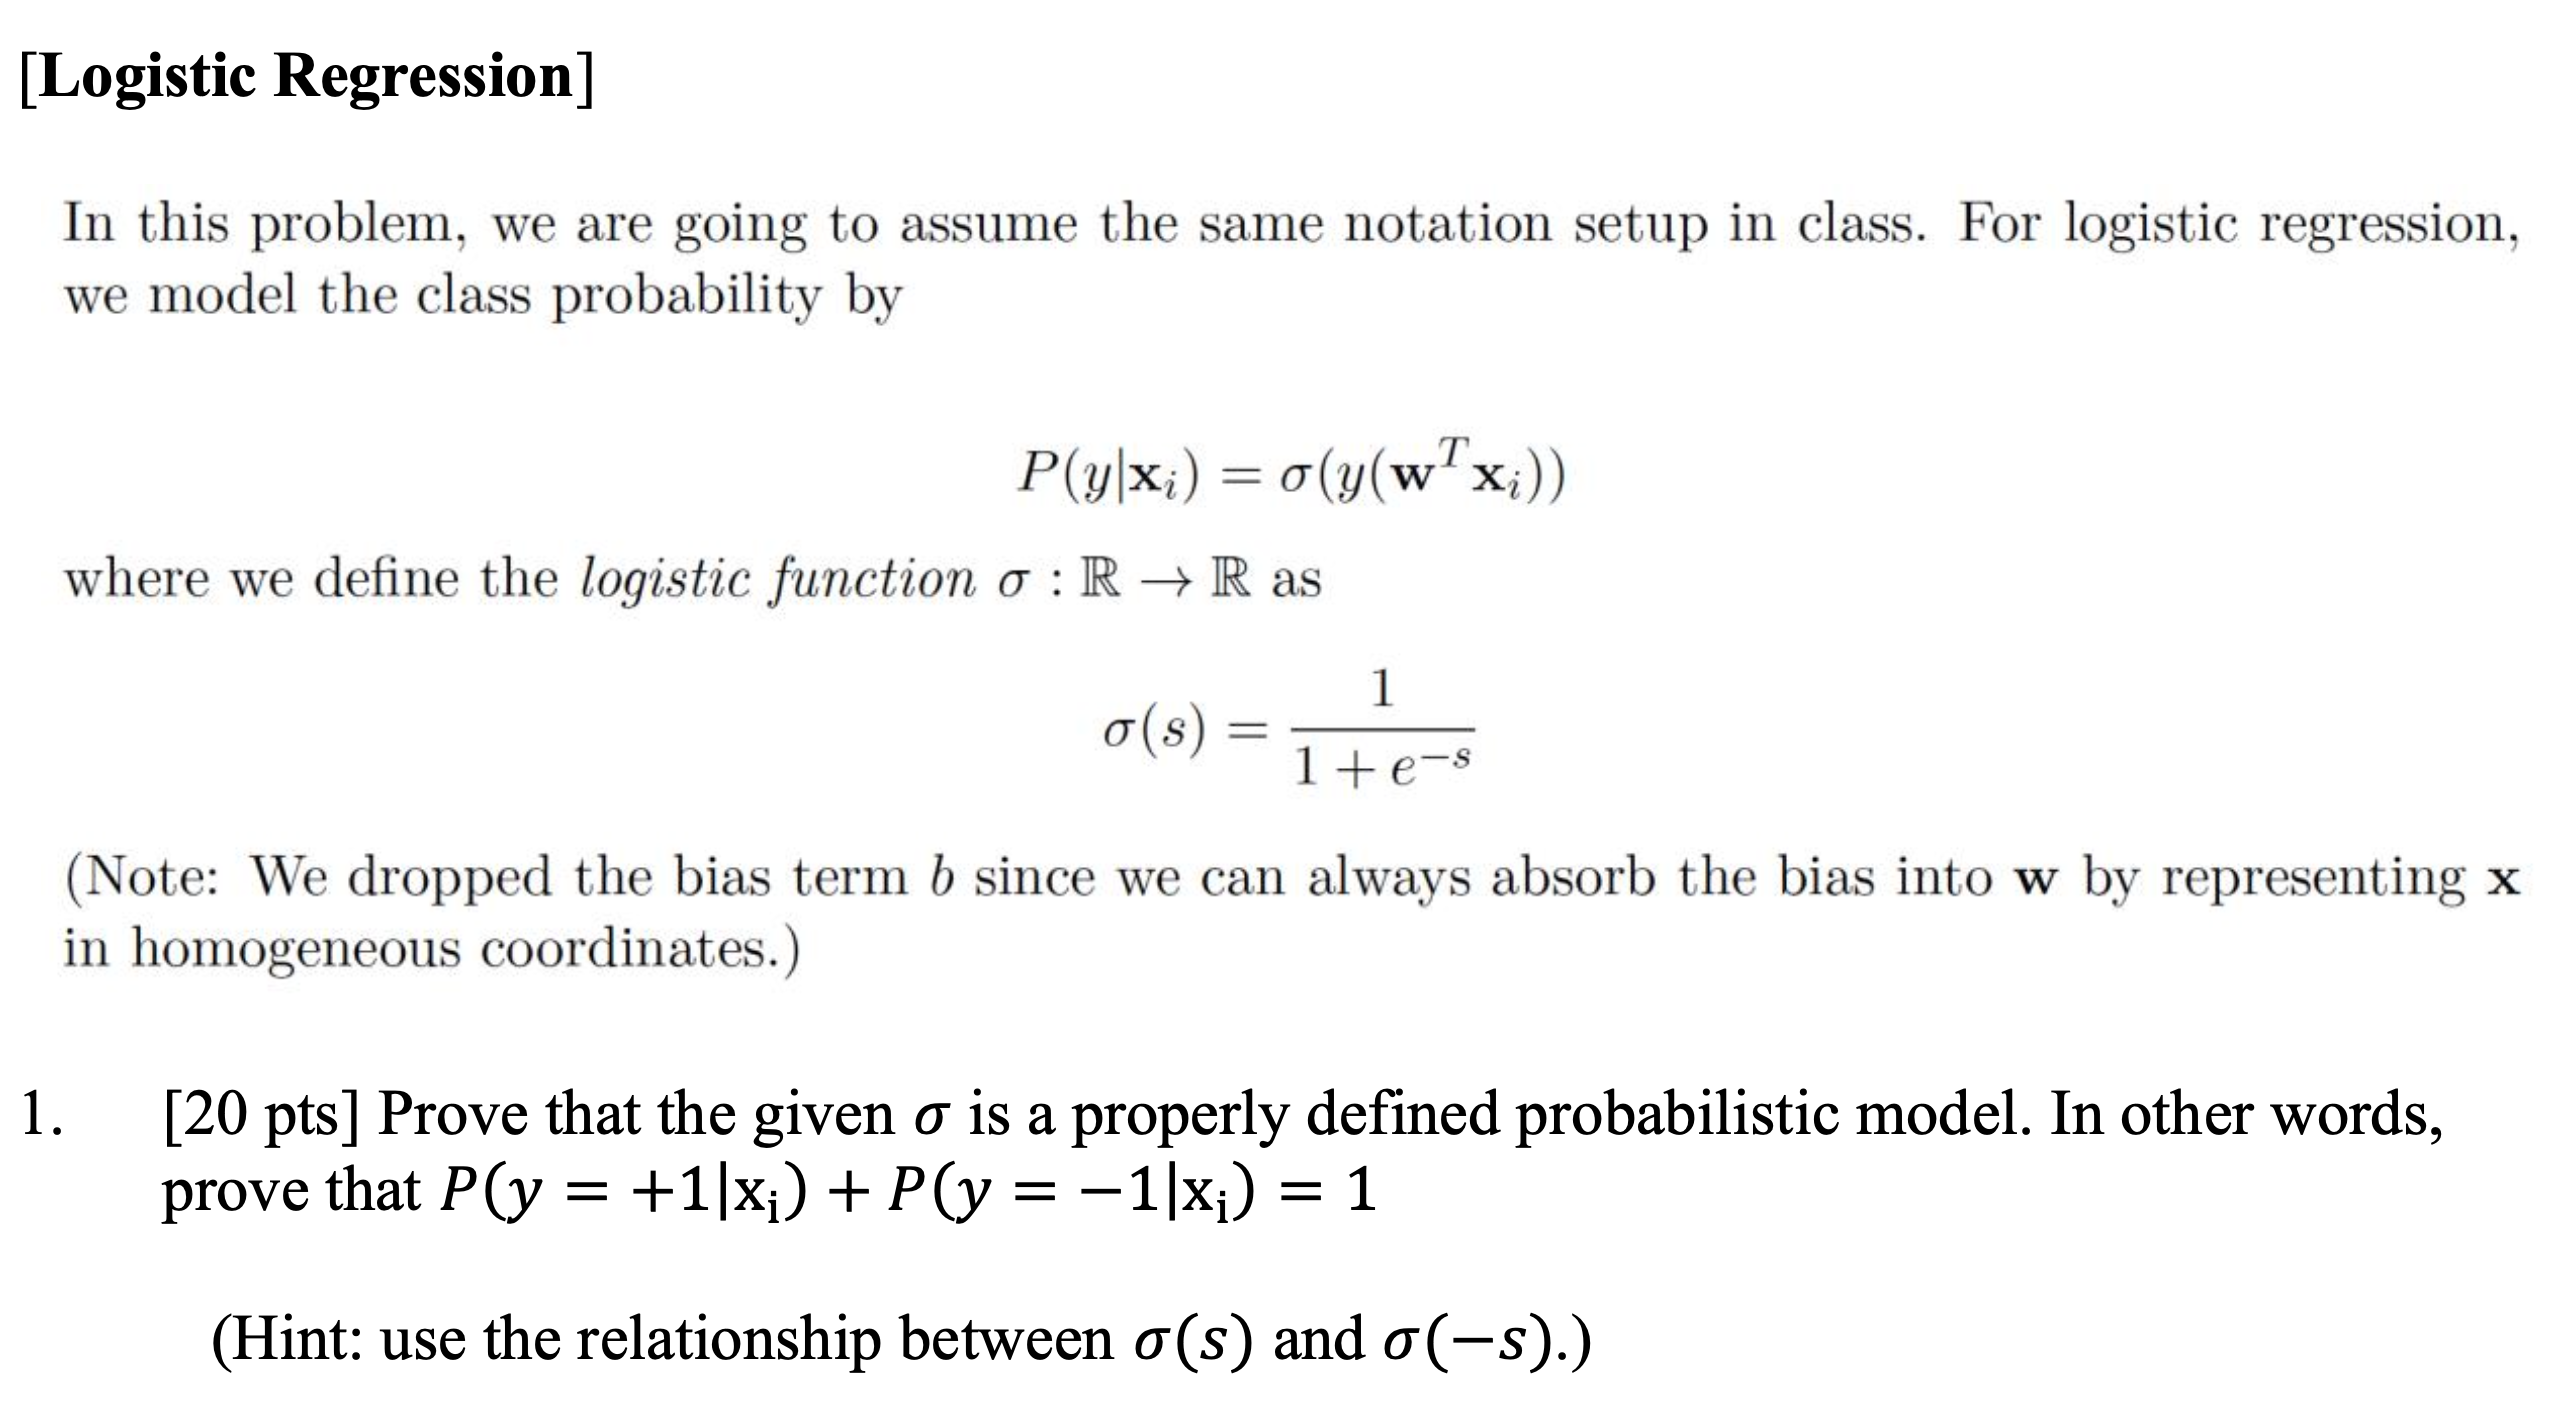
\includegraphics[width=1\textwidth]{media/hw4_q2.png}

Let's re-write $P(y|x_i)$ for each $y_i={-1,1}$ that we are given:

\begin{align}
    P(y=-1 | \mathbf{x_i}) &= \sigma(-1(\mathbf{w}^T \mathbf{x_i})) = \frac{1}{1+e^{\mathbf{w}^T \mathbf{x_i}}}\label{eq:q2_1}
\end{align} %&& \text{(from Eq. \ref{eq:hypothesis_class})}

\begin{align}
    P(y=1 | \mathbf{x_i}) &= \sigma(1(\mathbf{w}^T \mathbf{x_i})) = \frac{1}{1+e^{-\mathbf{w}^T \mathbf{x_i}}} \label{eq:q2_2} 
\end{align} %&& \text{(from Eq. \ref{eq:hypothesis_class})}

From our lectures, we know:

\begin{align}
    \sigma (s) &= 1 - \sigma(-s) \label{eq:q2_3} \nonumber \\
    \Rightarrow 1 &= \sigma(s) + \sigma(-s)
\end{align} %&& \text{(from Eq. \ref{eq:hypothesis_class})}

Then: 
\begin{align}
    1 &= \sigma(s) + \sigma(-s) \label{eq:q2_4} \nonumber \\
    &= \frac{1}{1+e^{-s}} + \frac{1}{1+e^{s}} 
\end{align}

We note that Equations \ref{eq:q2_1} and \ref{eq:q2_2} are of the form $\sigma(-s)$ for $y=-1$ and $\sigma(s)$ for $y=1$ respectively. Let's simplify and let $s = \mathbf{w}^T \mathbf{x_i}$. Then:

\begin{align}
    1 &= \frac{1}{1+e^{-s}} + \frac{1}{1+e^{s}}  \label{eq:q2_5} \nonumber \\
    &= \frac{(1+e^{s})+(1+e^{-s})}{(1+e^{-s})(1+e^{s})} \nonumber \\
    &= \frac{2+e^{s}+e^{-s}}{1+e^{-s}+e^{s}+e^{-s} \cdot e^{s}} \nonumber \\
    &= \frac{2+e^{s}+e^{-s}}{1+e^{-s}+e^{s}+1} && \text{(since $e^{-x} \cdot e^{x} = 1$)}\nonumber \\
    &= \frac{2+e^{s}+e^{-s}}{2+e^{s}+e^{-s}} \nonumber \\
    &=1
\end{align}

$\therefore$ Since $1 = \sigma(s) + \sigma(-s)$, where $s = \mathbf{w}^T \mathbf{x_i}$, then we have:

\begin{align}
    1 &= \sigma(\mathbf{w}^T \mathbf{x_i}) + \sigma(-\mathbf{w}^T \mathbf{x_i})  \label{eq:q2_6} 
\end{align}

Eq. \ref{eq:q2_6} corresponds to:
\begin{align}
    1 &= P(y=-1 | \mathbf{x_i}) + P(y=1 | \mathbf{x_i})  \label{eq:q2_7} 
\end{align}

$\therefore$ $\sigma$ is a properly-defined probabalistic model.

\subsection{Question Three}
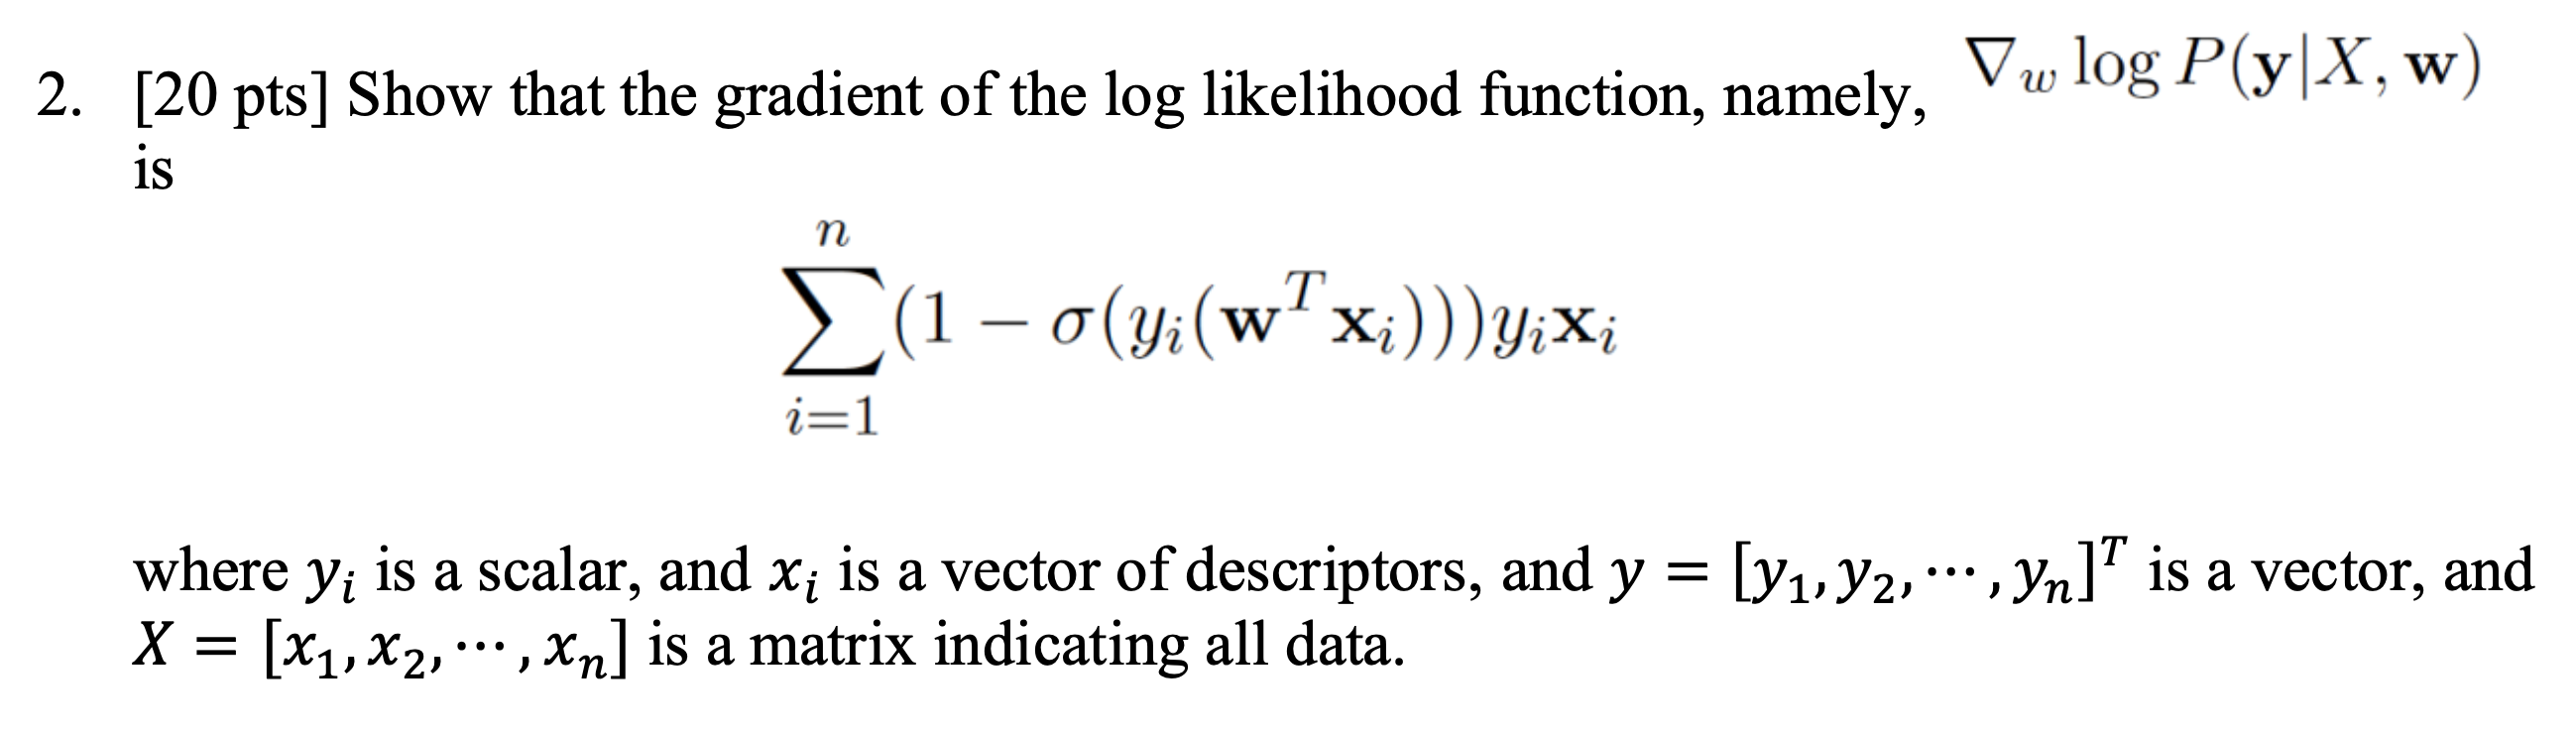
\includegraphics[width=1\textwidth]{media/hw4_q3.png}